\appendix
\renewcommand{\thesection}{\Alph{section}}
\setcounter{table}{0}
\renewcommand{\thetable}{A\arabic{table}} % Switch numbering to A1, A2, ...
\setcounter{figure}{0}
\renewcommand{\thefigure}{A\arabic{figure}} % Switch numbering to A1, A2, ...

% \section*{[Re] Don't Judge an Object by Its Context: Learning to Overcome Contextual Bias}

\section*{Appendix}

We dedicate the appendix to providing more details on certain parts of the main paper.
\begin{itemize}[leftmargin=*,noitemsep]
    \item In Section~\ref{sec:datasets}, we describe how we obtained and processed the four datasets.
    \item In Section~\ref{sec:biasedcategoriesapp}, we provide additional details on biased categories identification.
    \item In Section~\ref{sec:hyperparametersearch}, we describe our hyperparameter search.
    \item In Section~\ref{sec:epochselection}, we discuss different model selection methods we tried while reproducing the \textit{standard} baseline.
    \item In Section~\ref{sec:computationalrequirements}, we provide more details on computational requirements.
    \item In Section~\ref{sec:additionalresults}, we provide visualizations of DeepFashion and AwA results.
    \item In Section~\ref{sec:qualitative}, we provide additional qualitative analyses with CAMs.
    \item In Section~\ref{sec:percategory}, we provide per-category results for COCO-Stuff, DeepFashion, Animals with Attributes, and UnRel.
    \item In Section~\ref{sec:reproducibilityplan}, we provide the reproducibility plan we wrote at the start of the project.
\end{itemize}

\section{Datasets} \label{sec:datasets}

In this section, we describe how we obtained and processed the four datasets used in the paper. COCO-Stuff~\cite{caesar2018cvpr} and UnRel~\cite{Peyre17} are used for the object classification task, and DeepFashion~\cite{liuLQWTcvpr16DeepFashion} and Animals with Attributes~\cite{AwA} are used for the attribute classification task. COCO-Stuff is the main dataset used for discussion of quantitative and qualitative results. UnRel is used for cross-dataset experiments, i.e. testing models trained on COCO-Stuff on UnRel without fine-tuning.

\subsection{COCO-Stuff}
We downloaded COCO-Stuff~\cite{caesar2018cvpr} from the official homepage: \url{https://github.com/nightrome/cocostuff}. COCO-Stuff includes all 164K images from COCO-2017 (train 118K, val 5K, test-dev 20K, test-challenge 20K), but only the training and validation set annotations are publicly available. It covers 172 classes: 80 thing classes, 91 stuff classes and 1 class designated `unlabeled.'\\
\\
COCO-Stuff (COCO-2017 with ``stuff" annotations added) contains the same images as COCO-2014~\cite{COCO} but has different train-val-test splits. The original paper follows the data split of COCO-2014 and uses 82,783 images for training and 40,504 images for evaluation. The image numbers are consistent between COCO-2014 and COCO-2017, so we were able to map the ``stuff" annotations from COCO-Stuff to the COCO-2014 images with ``thing" annotations. Excluding the `unlabeled' category, we have in total 171 categories.\\
\\
In Table~\ref{tab:coco-data}, we report the co-occurrence, exclusive, and other counts for the paper's 20 biased category pairs. The co-occurrence count is the number of images where $b$ and $c$ co-occur; the exclusive count is the number of images where $b$ occurs without $c$; the other count is the number of remaining images where $b$ doesn't occur.\\
\\
During our data processing, we found a small typo in the original paper. Section 3 of the paper says ``COCO-Stuff has 2,209 images where `ski' co-occurs with `person,' but only has 29 images where `ski' occurs without `person.'" On the other hand, we found 2,180 co-occurring and 29 exclusive images in the training set. We verified with the authors that our data processing was correct. Merging COCO-2014 and COCO-Stuff annotations is a nontrivial step in the pipeline. We hope our published code and the Table~\ref{tab:coco-data} help future use.

\subsection{DeepFashion}
We downloaded DeepFashion~\cite{liuLQWTcvpr16DeepFashion} by following in the instructions on the official homepage: \url{http://mmlab.ie.cuhk.edu.hk/projects/DeepFashion.html}. The dataset consists of 5 benchmarks, out of which we use the Category and Attribute Prediction Benchmark. This benchmark consists of 209,222 training images, 40,000 validation images, and 40,000 test images with 1,000 attribute classes in total. Per the procedure specified by the authors, we only use the 250 most commonly appearing attributes. In Table~\ref{tab:deepfashion-data}, we report the co-occur, exclusive and other counts for the paper's 20 biased category pairs. It should be noted that the DeepFashion dataset was updated with additional ``fine-grained attribute annotations" in May 2020.

\subsection{Animals with Attributes}
Animals with Attributes (AwA)~\cite{AwA} is suspended and the images are no longer available because of copyright restrictions, according to the official homepage: \url{https://cvml.ist.ac.at/AwA/}. Hence we downloaded Animals with Attributes 2 (AwA2), which is described as a ``drop-in replacement" to AwA as it has the same class structure and almost the same characteristics, from the AwA2 official homepage: \url{https://cvml.ist.ac.at/AwA2/}. We confirmed with the authors that they used AwA2 as well. AwA2 consists of 30,337 training images with 40 animal classes and 6,985 test images with 10 other animal classes, with pre-extracted feature representations for each image. The classes are aligned with Osherson's classical class/attribute matrix, thereby providing 85 numeric attribute values for each class. The images were collected from public sources, such as Flickr, in 2016.\\
\\
In Table~\ref{tab:awa-data}, we report the co-occurrence, exclusive, and other counts for the paper's 20 biased category pairs. Following the description in the paper, we trained all models on the training set (40 classes) and evaluate on the test set (10 classes). 
For biased categories identification, following the paper description, we used the test set to determine the biased categories as these two sets contain different attribute distributions.

\subsection{UnRel}
We downloaded UnRel~\cite{Peyre17} from the official homepage: \url{https://github.com/jpeyre/unrel}. This dataset contains 1,071 images of objects out of their typical context and serves as a stress test for the models trained on COCO-Stuff. According to the paper, there are only three categories in UnRel that are shared with the 20 biased categories found in COCO-Stuff. We determined these categories to be ``skateboard," ``car" and ``bus." Only these three categories were used in the evaluation. 

\setlength{\textfloatsep}{10pt}

\begin{table}[b!]
\centering
\resizebox{\linewidth}{!}{
\begin{tabular}{|cc|cc|cc|cc||ccc|}
\hline
\multicolumn{2}{|c|}{Biased category pairs} & \multicolumn{2}{|c|}{Bias} & \multicolumn{2}{|c|}{Training (82,783)} & \multicolumn{2}{|c||}{Test (40,504)} & \multicolumn{3}{|c|}{Biased category pairs (Ours)} \\
\hline
Biased ($b$) & Context ($c$) & Paper & Ours & Co-occur & Exclusive & Co-occur & Exclusive & Biased ($b$) & Context ($c$) & Bias \\
\hline
cup            & dining table & 1.76   & 1.85 & 3,186 & 3,140 & 1,449 & 1,514 & car & road & 1.73 \\
wine glass     & person       & 1.80   & 1.59 & 1,151 & 583 & 548 & 304 & potted plant & furniture-other & 1.75 \\ 
handbag        & person       & 1.81   & 2.25 & 4,380 & 411 & 2,035 & 209 & spoon & bowl & 1.75 \\ 
apple          & fruit        & 1.91   & 2.12 & 477 & 627 & 208 & 244 & fork & dining table & 1.78 \\ 
car            & road         & 1.94   & 1.73 & 5,794 & 2,806 & 2,842 & 1,331 & bus & road & 1.79 \\ 
bus            & road         & 1.94   & 1.79 & 2,283 & 507 & 1,090 & 259 & cup & dining table & 1.85 \\ 
potted plant   & vase         & 1.99   & 1.73 & 930 & 2,152 & 482 & 1,058 & mouse & keyboard & 1.87 \\ 
spoon          & bowl         & 2.04   & 1.75 & 1,314 & 954 & 638 & 449 & remote & person & 1.89 \\ 
microwave      & oven         & 2.08   & 1.59 & 632 & 450 & 291 & 217 & wine glass & dining table & 1.94 \\ 
keyboard       & mouse        & 2.25   & 2.11 & 860 & 601 & 467 & 278 & clock & building-other & 1.97 \\ 
skis           & person       & 2.28   & 2.21 & 2,180 & 29 & 984 & 9 & keyboard & mouse & 2.11 \\ 
clock          & building     & 2.39   & 1.97 & 1,410 & 1,691 & 835 & 840 & apple & fruit & 2.12 \\ 
sports ball    & person       & 2.45   & 3.61 & 2,607 & 105 & 1,269 & 55 & skis & snow & 2.22 \\ 
remote         & person       & 2.45   & 1.89 & 1,469 & 666 & 656 & 357 & handbag & person & 2.25 \\ 
snowboard      & person       & 2.86   & 2.40 & 1,146 & 22 & 522 & 11 & snowboard & person & 2.40 \\ 
toaster        & ceiling\tablefootnote{We found this vague as there are two ceiling categories in COCO-Stuff: ceiling-other and ceiling-tile. We interpreted it as ceiling-other as ceiling-tile doesn't frequently co-occur with toaster.} & 3.70 & 1.98 & 60 & 91 & 30 & 44 & skateboard & person & 3.41 \\ 
hair drier     & towel        & 4.00   & 3.49 & 54 & 74& 28 & 41 & sports ball & person & 3.61 \\ 
tennis racket  & person       & 4.15   & 1.26 & 2,336 & 24 & 1,180 & 10 & hair drier & sink & 6.11 \\ 
skateboard     & person       & 7.36   & 3.41 & 2,473 & 38 & 1,068 & 24 & toaster & oven & 8.56 \\ 
baseball glove & person       & 339.15 & 31.32 & 1,834 & 19 & 820 & 9 & baseball glove & person & 31.32 \\ 
\hline
\end{tabular}
}
\vspace{0.1cm}
\caption{(Left) The paper's 20 most biased category pairs for \textbf{COCO-Stuff} and their bias values, both what's reported in the paper and what we've calculated with our trained model. (Middle) The number of co-occuring and exclusive images for each pair. (Right) The 20 most biased categories we've identified with our trained model.}
\label{tab:coco-data}
\end{table}

\begin{table}[bh!]
\centering
\resizebox{\linewidth}{!}{
\begin{tabular}{|cc|cc|cc|cc||ccc|}
\hline
\multicolumn{2}{|c|}{Biased category pairs} & \multicolumn{2}{|c|}{Bias} & \multicolumn{2}{|c|}{Training (209,222)} & \multicolumn{2}{|c||}{Test (40,000) } & \multicolumn{3}{|c|}{Biased category pairs (Ours)} \\
\hline
Biased ($b$) & Context ($c$) & Paper & Ours & Co-occur & Exclusive & Co-occur & Exclusive & Biased ($b$) & Context ($c$) & Bias \\
\hline
bell       & lace       & 3.15 & 2.74 & 167   & 549   & 32 & 92 & boyfriend & distressed & 3.35 \\
cut        & bodycon    & 3.30 & 3.46 & 313   & 2612  & 58 & 488 & gauze & embroidered & 3.35 \\ 
animal     & print      & 3.31 & 2.29 & 592   & 234   & 106 & 52 & la & muscle & 3.35 \\ 
flare      & fit        & 3.31 & 2.56 & 2,960 & 527   & 561 & 103 & diamond & print & 3.40\\ 
embroidery & crochet    & 3.44 & 3.04 & 237   & 1,021 & 42 & 221 & york & city & 3.43 \\ 
suede      & fringe     & 3.48 & 2.75 & 104   & 478   & 23 & 92 & retro & chiffon & 3.43 \\ 
jacquard   & flare      & 3.68 & 4.02 & 71    & 538   &  11 & 107 & cut  & bodycon  & 3.46 \\ 
trapeze    & striped    & 3.70 & 2.85 & 51    & 531   &  14 & 127 & fitted  & sleeve  & 3.58  \\ 
neckline   & sweetheart & 3.98 & 3.16 & 161   & 818   &  25 & 156 & light  & wash &  3.59\\ 
retro      & chiffon    & 4.08 & 3.43 & 119   & 1,135 & 26 & 224 & sequin  & mini  & 3.63 \\ 
sweet      & crochet    & 4.32 & 6.55 & 180   & 1,122 &  29 & 190 & cuffed &  denim  & 3.70 \\ 
batwing    & loose      & 4.36 & 3.89 & 181   & 518   &  40 & 100 & lady &  chiffon  & 3.71  \\ 
tassel     & chiffon    & 4.48 & 3.15 & 71    & 651   &  8 & 131  & jacquard &  fit &  4.02 \\ 
boyfriend  & distressed & 4.50 & 3.35 & 276   & 1,172 & 63 & 215 & bell  & sleeve &  4.23 \\ 
light      & skinny     & 4.53 & 3.31 & 216   & 1,621 & 47 & 298 & ankle &  skinny &  4.42 \\ 
ankle      & skinny     & 4.56 & 4.42 & 340   & 462   &  68 & 96 &  tiered &  crochet &  4.45 \\ 
french     & terry      & 5.09 & 7.64 & 975   & 646   &  178 & 121 & studded  & denim  & 4.98 \\ 
dark       & wash       & 5.13 & 5.66 & 343   & 1,011 &  69 & 191 & dark  & wash  & 5.66 \\ 
medium     & wash       & 7.45 & 6.78 & 227   & 653   & 35 & 153  & sweet  & crochet  & 6.55  \\ 
studded    & denim      & 7.80 & 4.98 & 139   & 466   & 25 & 95 & medium  & wash  & 6.78\\ 

\hline
\end{tabular}
}
\vspace{0.1cm}
\caption{(Left) The paper's 20 most biased category pairs for \textbf{DeepFashion} and their bias values, both what's reported in the paper and what we've calculated with our trained model. (Middle) The number of co-occuring and exclusive images for each pair. (Right) The 20 most biased categories we've identified with our trained model.}
\label{tab:deepfashion-data}
\end{table}



\section{Biased categories identification}
\label{sec:biasedcategoriesapp}

In this section, we provide additional details on the biased categories identification process discussed in Section~\ref{sec:biasedcategories} of the main paper.\\
\\
For each dataset, the paper identifies the top-20 $(b, c)$ pairs of biased categories, where $b$ is the category suffering from contextual bias and $c$ is the associated context category. For a given category $z$, let $\mathbb{I}_b \cap \mathbb{I}_z$ and $\mathbb{I}_b \setminus \mathbb{I}_z$ denote sets of images where $b$ occurs with and without $z$ respectively. Let $\hat{p}(I, b)$ denote the prediction probability of an image $I$ for a category $b$ obtained from a trained multi-class classifier. The \textit{bias} between two categories $b$ and $z$ is defined as follows:
\begin{equation}
    \text{bias}(b,z)=\frac{\frac{1}{|\mathbb{I}_b \cap \mathbb{I}_z|} \sum_{I\in \mathbb{I}_b \cap \mathbb{I}_z} \hat{p}(I,b)}{\frac{1}{|\mathbb{I}_b \setminus \mathbb{I}_z|} \sum_{I\in \mathbb{I}_b \setminus \mathbb{I}_z} \hat{p}(I,b)},
\end{equation}
which is the ratio of average prediction probabilities of $b$ when it occurs with and without $z$. The category $c$ that most biases $b$ is determined as $c = \arg \max_z \text{bias}(b, z)$, with a condition that they co-occur frequently. Specifically, the paper defines that $b$ must co-occur at least 20\% of the time with $c$ for COCO-Stuff and AwA, and 10\% for DeepFashion. 
In short, a given category $b$ is most biased by $c$ if (1) $b$ co-occurs frequently with $c$ and (2) the prediction probability of $b$ drop significantly in the \textit{absence} of $c$.\\
\\
While this method can be applied to any number of biased category pairs, the paper says using $K$=20 sufficiently captures biased categories in all datasets used the paper. 
We report the 20 most biased category pairs we've identified and compare them to those identified by the paper in Tables~\ref{tab:coco-data} (COCO-Stuff),~\ref{tab:deepfashion-data} (DeepFashion),~\ref{tab:awa-data} (AwA). We discuss the results for each dataset in more detail below.\\

\begin{table}[t!]
\centering
\caption{(Left) The paper's 20 most biased category pairs for \textbf{AwA} and their bias values, both what's reported in the paper and what we've calculated with our trained model. (Middle) The number of co-occuring and exclusive images for each pair. (Right) The 20 most biased categories we've identified with our trained model.}
\label{tab:awa-data}
\resizebox{\linewidth}{!}{
\begin{tabular}{|cc|cc|cc|cc||ccc|}
\hline
\multicolumn{2}{|c|}{Biased category pairs} & \multicolumn{2}{|c|}{Bias} & \multicolumn{2}{|c|}{Training (30,337)} & \multicolumn{2}{|c||}{Test (6,985)} & \multicolumn{3}{|c|}{Biased category pairs (Ours)} \\
\hline
Biased ($b$) & Context ($c$) & Paper & Ours & Co-occur & Exclusive & Co-occur & Exclusive & Biased ($b$) & Context ($c$) & Bias \\
\hline
white     & ground    & 3.67   &   4.08  & 12,952 & 1,237  & 3,156 & 988   & forager     & nestspot  &   4.04 \\
longleg   & domestic  & 3.71   &   6.55  & 3,727  & 7,667  & 728   & 720   & white       & ground    &   4.08 \\ 
forager   & nestspot  & 4.02   &   4.04  & 7,740  & 7,214  & 3,144 & 713   & hairless    & swims     &   4.29 \\ 
lean      & stalker   & 4.46   &   3.91  & 5,312  & 11,592 & 720   & 1,038 & muscle      & black     &   4.63 \\ 
fish      & timid     & 5.14   &   6.30  & 2,786  & 2,675  & 4,002 & 1,232 & insects     & gray      &   4.97 \\ 
hunter    & big       & 5.34   &   8.99  & 6,557  & 3,207  & 1,708 & 310   & fish        & timid     &   6.30 \\ 
plains    & stalker   & 5.40   &   1.81  & 3,793  & 12,865 & 720   & 310   & longleg     & domestic  &   6.55 \\ 
nocturnal & white     & 5.84   &   6.97  & 3,118  & 2,464  & 822   & 720   & nocturnal   & white     &   6.97 \\ 
nestspot  & meatteeth & 5.92   &   8.14  & 4,788  & 5,180  & 2,270 & 874   & nestspot    & meatteeth &   8.14 \\ 
jungle    & muscle    & 6.26   &   9.15  & 4,480  & 696    & 2,132 & 874   & hunter      & big       &   8.99 \\ 
muscle    & black     & 6.39   &   4.63  & 10,656 & 8,960  & 2,157 & 684   & jungle      & muscle    &   9.15 \\ 
meat      & fish      & 7.12   &  10.17  & 3,175  & 7,819  & 1,979 & 310   & meat        & fish      &  10.17 \\ 
mountains & paws      & 9.24   &  14.74  & 3,090  & 4,897  & 1,232 & 728   & domestic    & inactive  &  11.02 \\ 
tree      & tail      & 10.98  &  11.48  & 2,121  & 1,255  & 1,960 & 874   & tree        & tail      &  11.48 \\ 
domestic  & inactive  & 11.77  &  11.02  & 5,853  & 5,953  & 3,322 & 728   & spots       & longleg   &  12.50 \\ 
spots     & longleg   & 20.15  &  12.50  & 3,095  & 2,433  & 720   & 3,087 & mountains   & paws      &  14.74 \\ 
bush      & meat      & 29.47  &  31.26  & 1,896  & 5,922  & 6,265 & 1,602 & bush        & meat      &  31.26 \\ 
buckteeth & smelly    & 34.01  &  51.25  & 3,701  & 3,339  & 310   & 874   & buckteeth   & smelly    &  51.25 \\ 
slow      & strong    & 76.59  &  125.19 & 8,710  & 1,708  & 3,968 & 747   & slow        & strong    & 125.19 \\ 
blue      & coastal   & 319.98 &1,393.25 & 946    & 174    & 709  & 747    & blue        & coastal   & 1,393.25 \\ 
\hline
\end{tabular}
}
\end{table}

\textbf{COCO-Stuff:} Overall, the bias values of the paper's biased category pairs calculated with our model are similar to the paper's values. Furthermore, most of our biased category pairs match with the paper's pairs. 18 of the 20 biased categories overlap, although their context categories sometimes differ. \\
\\
\textbf{DeepFashion:} After manual cleaning per suggestion of the authors, 10 of our biased category pairs match with the paper's. Still, the bias values of the paper's pairs calculated with our trained model are overall similar to the paper's values. It is worth noting that there are fewer co-occurring and exclusive images for each of the biased category pairs, compared to COCO-Stuff.\\
\\
\textbf{Animals with Attributes:} Almost all of our biased categories match with those in the paper. However, we observed in the process of determining the biased categories that for each $b$, there were multiple categories $c$ which had an equally biased effect on $b$. That is, the bias value $\text{bias}(b, c)$ was equal over each of these $c$'s. We suspect that this is because the images in AwA are labeled by animal class rather than per image, so many images share the same exact labels. Moreover, we observed that for many image examples, the baseline model's highest prediction scores differ by less than 0.0001. The combination of these two events may result in extremely similar bias scores. Since there were multiple $c$'s for each $b$, we listed the category which matched the paper's findings whenever possible. In total, 18 of our biased categories overlapped with those in the paper.

\setlength{\textfloatsep}{20pt}

\section{Hyperparameter search} \label{sec:hyperparametersearch}

In this section, we describe how we conducted our hyperparameter search. The paper does not describe the hyperparameter search process, so we followed standard practice and tuned the hyperparameters on the validation set. While DeepFashion has training, validation and test sets, COCO-Stuff and AwA don't have validation sets, so we created a random 80-20 split of the original training set and used the 80 split as the training set and the 20 split as the validation set. We later confirmed with the authors that this is how they did their hyperparameter search.\\
\\
\textbf{Search for the ``stage 1" \textit{standard} model:} For COCO-Stuff, we tried varying the learning rate (0.1, 0.05, 0.01), weight decay (0, 1e-5, 1e-4, 1e-3), and the epoch after which learning rate is dropped (20, 40, 60). We found that the paper's hyperparameters (0.1 learning rate dropped to 0.01 after epoch 60 with no weight decay) produced the best results.
For DeepFashion, we varied the learning rate (0.1, 0.05, 0.01, 0.005, 0.001, 0.0001), weight decay (0, 1e-6, 1e-5, 1e-4), and the epoch after which the learning rate dropped (20, 30). We obtained the best results using a constant learning rate of 0.1 and weight decay of 1e-6.
For AwA, we tried learning rates of 0.1 and 0.01, with various training schedules such as dropping from 0.1 to 0.001, dropping from 0.01 to 0.001, and keeping a constant learning rate of 0.01 throughout. We also tried varying weight decay (0, 1e-2, 1e-3, 1e-4, 1e-5), but the paper's hyperparameters (0.1 learning rate dropped to 0.01 after epoch 10 with no weight decay) led to the best results.
We also tried training the models longer but didn't find much improvement, so we trained for the same number of epochs as in the paper (100 for COCO-Stuff, 50 for DeepFashion, 20 for AwA).\\
\\
\textbf{Search for the ``stage 2" models:} For ``stage 2" models, we tried varying the learning rate (0.005, 0.01, 0.05, 0.1, 0.5) and found that the paper's learning rate of 0.01 produces the best results. We didn't find benefits from training the models longer, so following the original authors, we train all ``stage 2" models (except \textit{split-biased}) for 20 epochs on top of the \textit{standard} model and use the model at the end of training as the final model. For the \textit{CAM-based} model, we conducted an additional hyperparameter search because we got underwhelming results and degenerate CAMs with the paper's hyperparameters ($\lambda_1$=0.1, $\lambda_2$=0.01). We tried varying the regularization weight $\lambda_2$ (0.01, 0.05, 0.1, 0.5, 1.0, 5.0) and achieved the best results with $\lambda_2$=0.1.


\section{Selecting the best model epoch} \label{sec:epochselection}

While reproducing the \textit{standard} model in Section~\ref{sec:baseline}, we tried selecting the best model epoch with four different selection methods: 1) lowest loss, 2) highest exclusive mAP, 3) highest combined exclusive and co-occur mAPs, and 4) last epoch (paper's method). Note that method 4 does not require a validation set, while methods 1-3 do as they require examinations of the loss and the mAPs at every epoch. Hence for datasets like COCO-Stuff and AwA that don't have a validation set, we can apply the first three methods only when we create a validation set by doing a random split of the original training set (e.g., 80-20 split).\\
\\
In Table~\ref{tab:epochselection}, we show COCO-Stuff \textit{standard} results with different epoch selection methods. For methods 1–3, the best epoch is selected based on the loss or the mAPs on the validation set. For method 4, we simply select the last epoch. Note that all numbers in the table are results on the unseen test set. \\
\\
First considering the model trained on the 80 split, we see that selecting the epoch with the lowest (BCE) loss yields the lowest mAP (row 1). The results of the other three methods (rows 2–4) are largely similar, with less than 0.4 mAP difference for all fields. When we plot the progression of the losses and the mAPs (Figure~\ref{fig:baselinetraining}), we see that the mAPs are mostly consistent in the latter epochs. Hence, we decided that using the last epoch is a reasonable epoch selection method. With this method we also benefit from training on the full training set, which improves all four mAPs (row 5).

\begin{table}[h!]
\centering
\caption{COCO-Stuff \textit{standard} baseline results with different model epoch selection methods. All numbers are results on the test set. The best results are in bold.}
\label{tab:epochselection}
\resizebox{\linewidth}{!}{
\begin{tabular}{|c|c|c|c|c|c|c|}
\hline
Training data & Selection method & Selected epoch & Exclusive & Co-occur & All & Non-biased \\
\hline
80 split & 1) Lowest loss & 36 & 22.0 & 64.0 & 55.4 & 71.8 \\
80 split & 2) Highest exclusive mAP & 79 & 22.9 & 64.1 & 55.2 & 71.6 \\
80 split & 3) Highest exclusive + co-occur mAP & 68 & 23.0 & 64.2 & 55.3 & 71.8 \\
80 split & 4) Last epoch & 100 & 22.9 & 63.8 & 55.0 & 71.4 \\
\hline
Full training set & 4) Last epoch & 100 & \textbf{23.9} & \textbf{65.0} & \textbf{55.7} & \textbf{72.3} \\
\hline
\end{tabular}
}
\end{table}

\begin{figure}[h!]
\centering
\caption{Losses and mAPs of the COCO-Stuff \textit{standard} model trained on the 80 split of the original training set. The validation loss and the four mAPs are calculated on the remaining 20 split which we use as the validation set.}
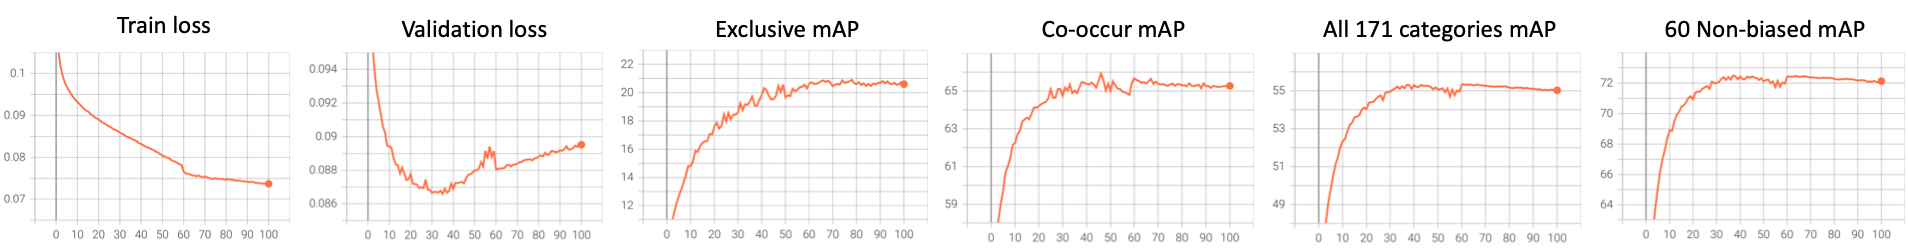
\includegraphics[width=\linewidth]{../openreview/images/baseline.png}
\label{fig:baselinetraining}
\end{figure}


\section{Computational requirements} \label{sec:computationalrequirements}

In Table~\ref{tab:trainingtime}, we report the single-epoch training time for each method trained with a batch size of 200 using a single RTX 3090 GPU, except for \textit{CAM-based} which is trained on two GPUs due to memory constraints. Overall, the total training time for each method range from 35-43 hours on COCO-Stuff, 22-29 hours on DeepFashion, and 7-8 hours on AwA.
For inference, a single image forward pass takes 9.5ms on a single RTX 3090 GPU. 
Doing inference on the entire test with a batch size of 100 takes 5.6 minutes for COCO-Stuff (40,504 images), 2.7 minutes for DeepFashion (40,000 images), 1.8 minutes for AwA (6,985 images), and 18.2 seconds for UnRel (1,071 images).

\begin{table}[h!]
\centering
\caption{Single-epoch training time (in minutes) for different methods using a batch size of 200.}
\label{tab:trainingtime}
\begin{tabular}{|c|ccc|}
\hline
Method & COCO-Stuff & DeepFashion & AwA  \\
\hline
\textit{standard}         & 12.9 & 16.8 & 8.8 \\
\hline
\textit{remove labels}    & 12.8 & 16.8 & 8.8 \\
\textit{remove images}    & 8.4  & 16.1 & 0.5 \\
\textit{split-biased}     & 12.9 & 16.7 & 8.8 \\
\textit{weighted}         & 12.9 & 16.8 & 8.8 \\
\textit{negative penalty} & 12.8 & 16.8 & 8.8 \\
\textit{class-balancing}  & 12.8 & 16.9 & 8.8 \\
\textit{attribute decorrelation}  & - & - & 12.8  \\
\hline
\textit{CAM-based}        & 17.3  & - & - \\
\textit{feature-split}    & 13.3 & 20.9 & 10.0\\
\hline
\end{tabular}
\end{table}


\section{Additional results} \label{sec:additionalresults}

In Figure~\ref{fig:mAPs-comparison}, we show visual comparisons of our results and the paper's results reported in Table~\ref{tab:mainresults} for the AwA and DeepFashion datasets. A similar plot for COCO-Stuff is presented in Figure~\ref{fig:COCOStuff-mAPs} of the main paper.

\begin{figure}[h!]
    \centering
    \caption{Performance of different methods on DeepFashion and AwA. The blue and red lines mark the paper's and our \textit{standard} mAPs. All results can be found in Table~\ref{tab:mainresults}.}
    \label{fig:mAPs-comparison}
    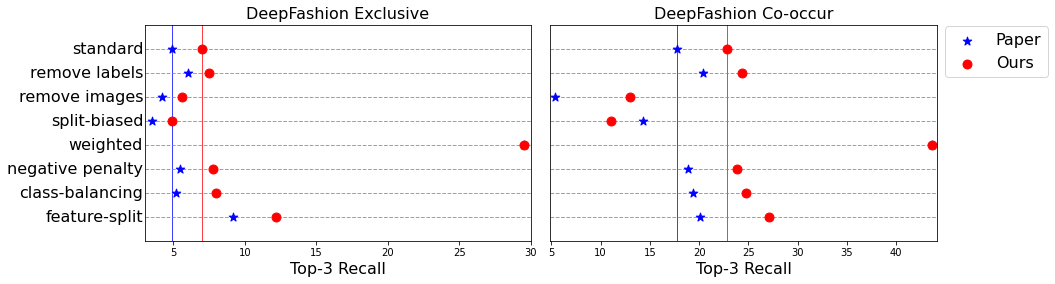
\includegraphics[width=\textwidth]{../openreview/images/DeepFashion_maP_comparisons.png}
    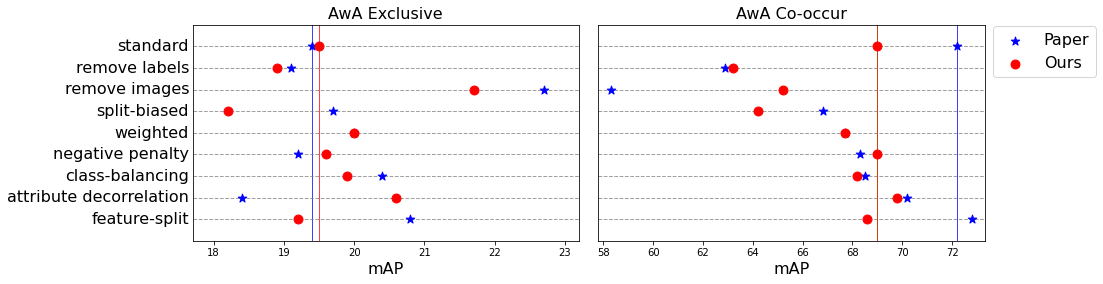
\includegraphics[width=\textwidth]{../openreview/images/AwA_maP_comparisons.png}
\end{figure}


% \addtolength{\textfloatsep}{0.2in}

\section{Additional qualitative analyses}
\label{sec:qualitative}

In Figures 6 through 9 of the original paper, the CAMs produced by the \textit{CAM-based} and \textit{feature-split} methods are compared to those of the \textit{standard} model. Since the image IDs of the images used in these figures were not made available, we attempted to find images that closely replicated those used in the paper.\\
\\
Figures 6 and 7 of the original paper compare the CAMs of the \textit{CAM-based} method against those of the \textit{standard} and \textit{feature-split} method. The paper's comparison between the \textit{CAM-based} and \textit{feature-split} models shows that the \textit{feature-split} CAM regions cover both $b$ and $c$ categories, whereas the \textit{CAM-based} model's CAM covers mostly the area of $b$. In the majority of our examples, we found this distinction to be less clear (Figure~\ref{fig:original_fig7}). Likewise, the CAMs of our \textit{CAM-based} method compared to the CAMs of our \textit{standard} model are also only slightly different, even on instances where the \textit{CAM-based} model succeeds but the \textit{standard} model fails (Figure~\ref{fig:original_fig6}).\\
\\
Figure 8 in the original paper gives several examples images in which the biased categories $b$ appear away from their context $c$. Specifically, there are examples for which the \textit{feature-split} model was able to predict $b$ correctly but the \textit{standard} model failed to do so, as well as some examples where both models failed. Figure~\ref{fig:original_fig8} shows some of our own examples. Several of the examples from the original paper also came up in our own analysis. Out of all the test images, we found 1 ``skateboard" examples on which our \textit{feature-split} model was successful but our \textit{standard} model failed, and 11 examples on which both models failed. There were 3 ``microwave" examples on which only \textit{feature-split} was successful and 131 examples on which neither model was successful. For ``snowboard", there were 4 examples on which only the \textit{feature-split} model was successful and 4 examples on which both failed.\\
\\
Figure 9 of the original paper shows how the CAMs derived from $W_o$ and $W_s$, the two halves of the \textit{feature-split} model's feature subspace, focus on the object $b$ and the context $c$, respectively. We noticed the same trend in our qualitative observations (Figure~\ref{fig:featuresplit-comparisons}).

\begin{figure}[h!]
    \centering
    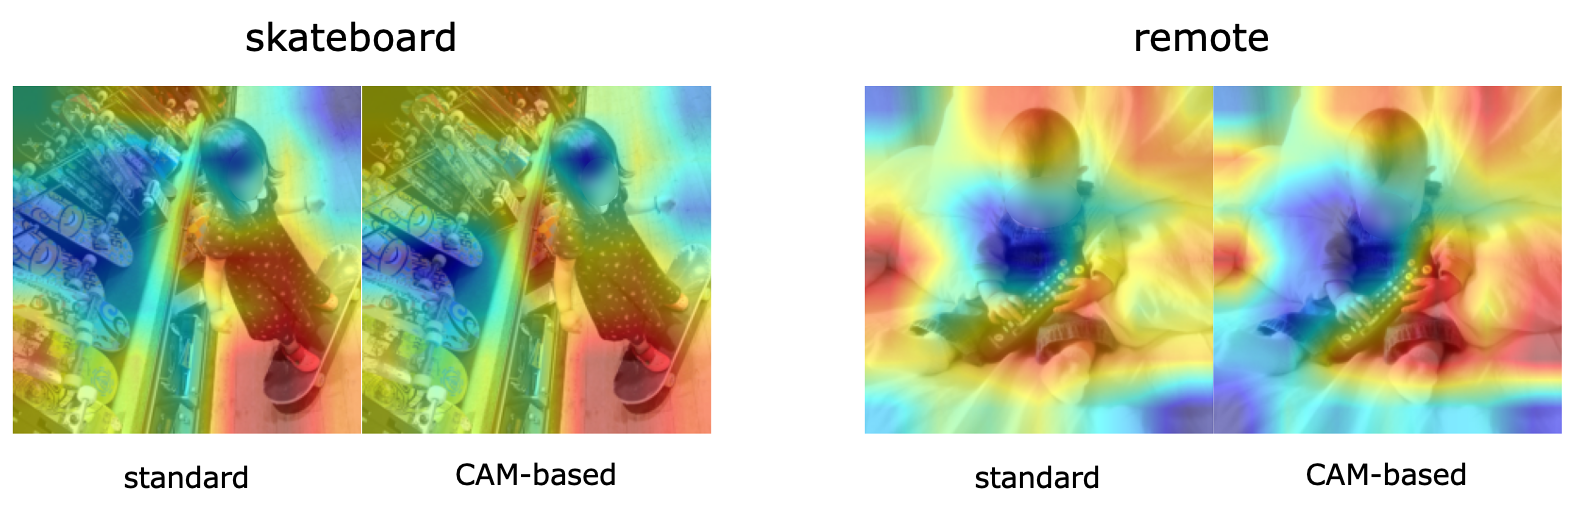
\includegraphics[width=\textwidth]{../openreview/images/figure6.png}
    \caption{CAMs of examples on which our \textit{CAM-based} model succeeds and our \textit{standard} model fails. They are visually quite similar.}
    \label{fig:original_fig6}
\end{figure}

\begin{figure}[h!]
    \centering
    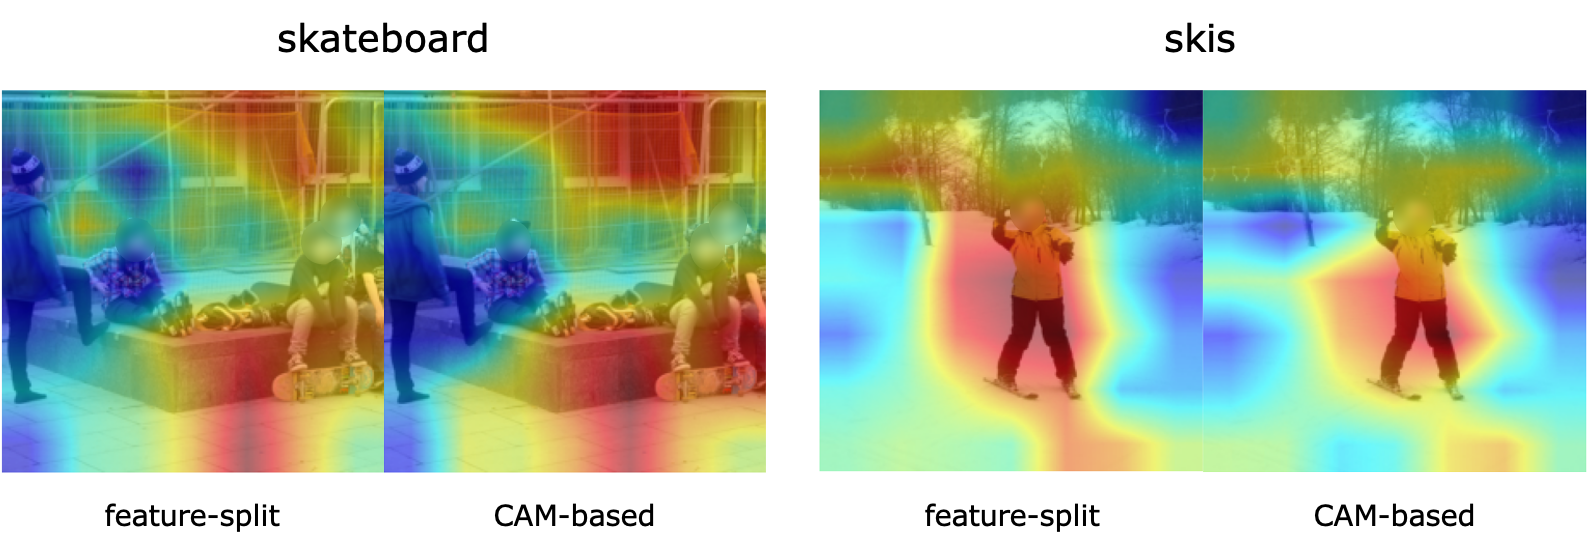
\includegraphics[width=\textwidth]{../openreview/images/fs_not_cam.png}
    \caption{CAMs of examples on which our \textit{feature-split} model succeeds and our \textit{CAM-based} model fails. They are visually quite similar.}
    \label{fig:original_fig7}
\end{figure}

\begin{figure}[h!]
    \centering
    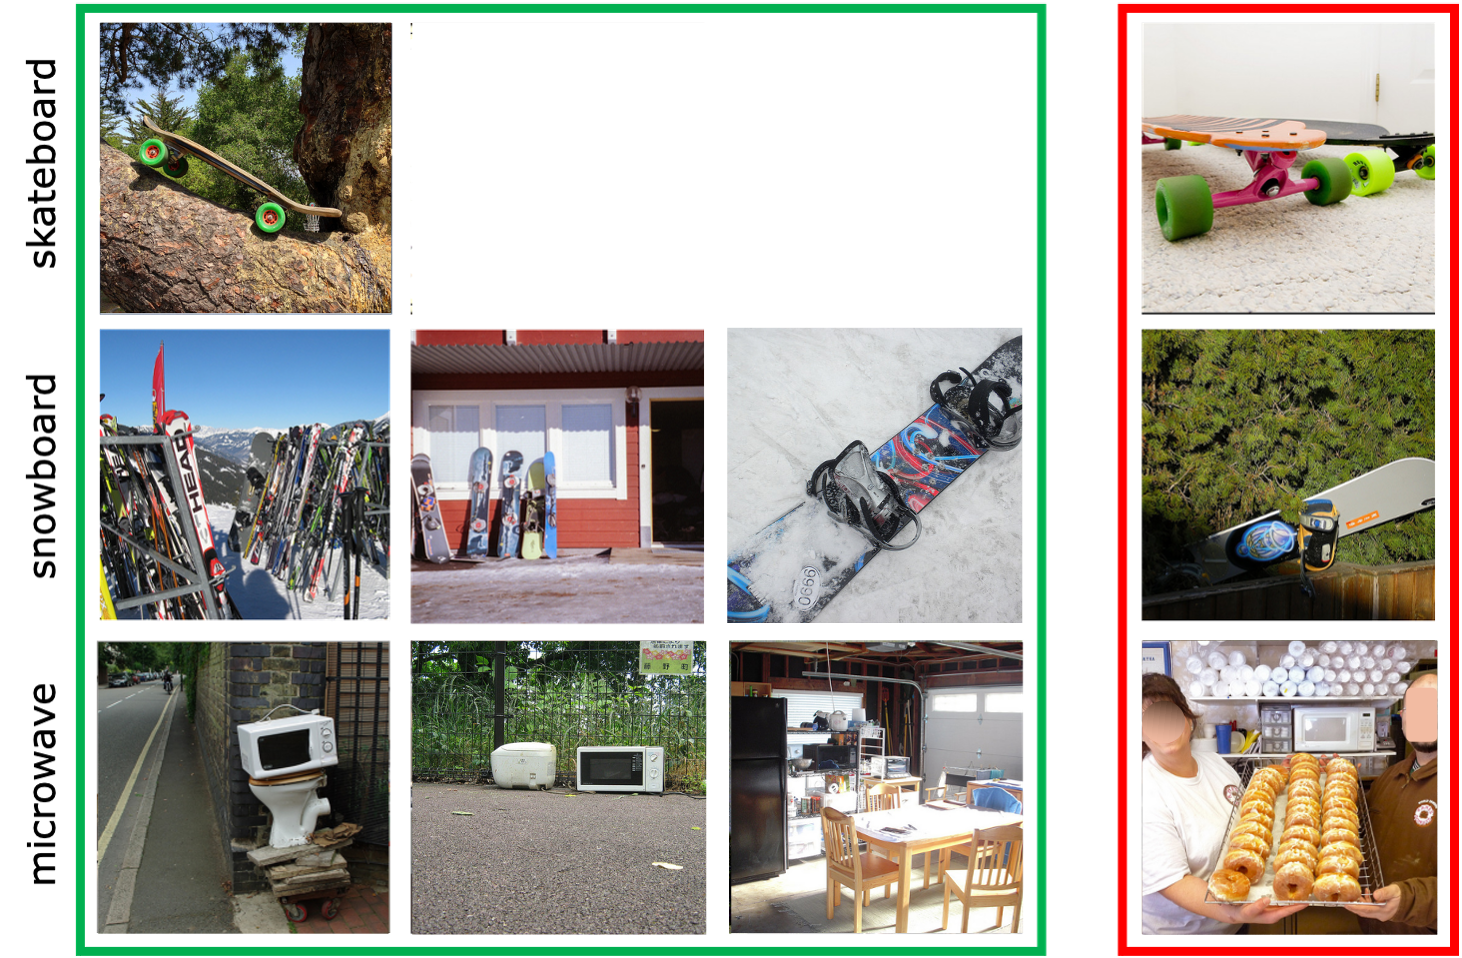
\includegraphics[width=\textwidth]{../openreview/images/figure8.png}
    \caption{Examples on which our \textit{feature-split} model succeeds and our  \textit{standard} model fails are outlined in green (left box). Examples on which both models fail are outlined in red (right box). While the original paper shows three examples of images containing \textit{skateboard} on which the \textit{feature-split} model succeeds but the \textit{CAM-based} model fails, we only found one.}
    \label{fig:original_fig8}
\end{figure}

\begin{figure}[h!]
    \centering
    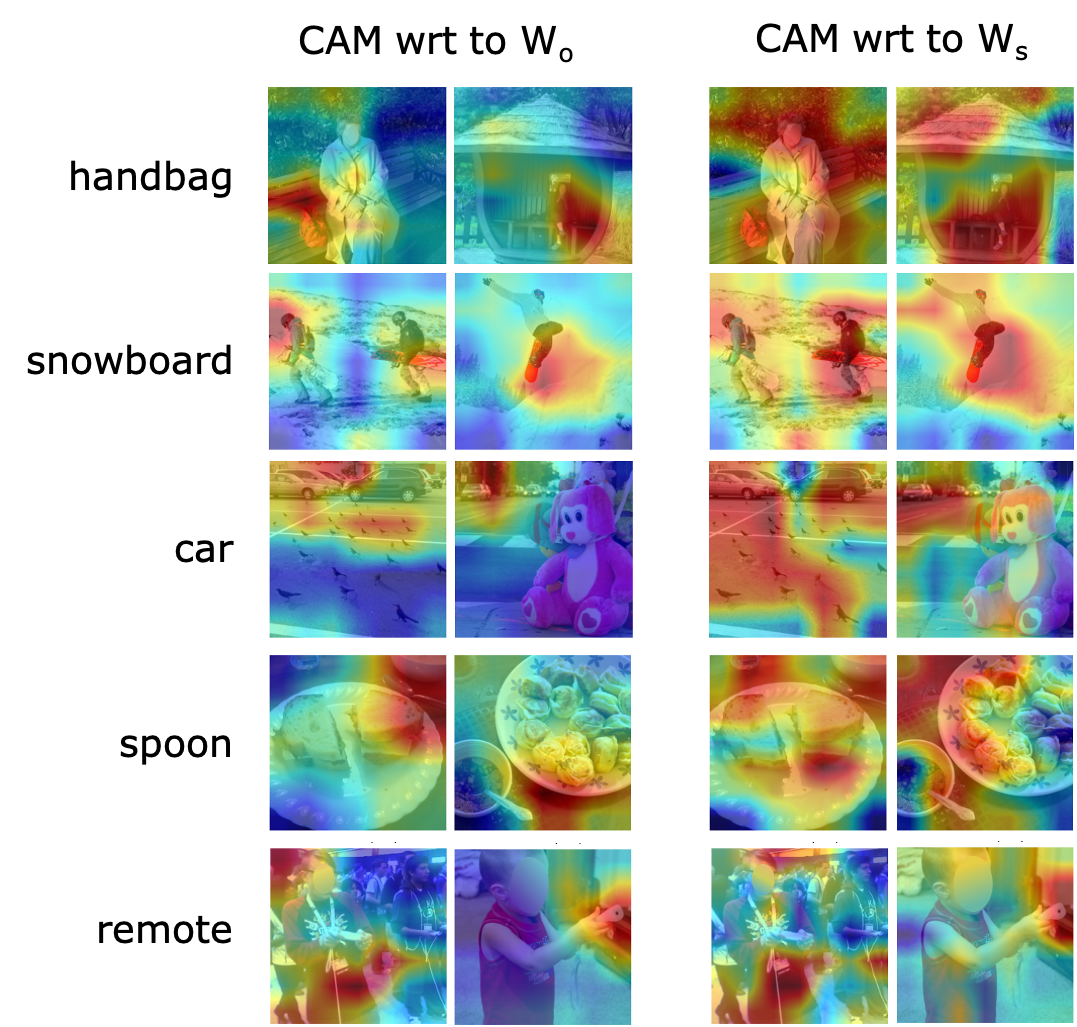
\includegraphics[width=0.9\textwidth]{../openreview/images/featuresplit-comparisons.png}
    \caption{Interpreting the \textit{feature-split} method by visualizing the CAMs with respect to $W_o$ and $W_s$. Consistent with the paper's observations, we see that $W_o$ focuses on the actual category (e.g., handbag, snowboard, car, spoon, remote) while $W_s$ looks at context (e.g.m person, road, bowl).}
    \label{fig:featuresplit-comparisons}
\end{figure}



\clearpage
\section{Per-category results}
\label{sec:percategory}

In Table~\ref{tab:mainresults}, we reported results aggregated over multiple categories. In this section, we present per-category results for the \textit{standard}, \textit{CAM-based}, and \textit{feature-split} methods in Tables~\ref{tab:coco-results} (COCO-Stuff),~\ref{tab:deepfashion-results} (DeepFashion), and~\ref{tab:awa-results} (AwA), and compare them to the paper's results. We also present our results on the UnRel dataset in Table~\ref{tab:unrel-results}.

\begin{table}[h]
\centering
\caption{Per-category results on \textbf{COCO-Stuff}. This table together with Table~\ref{tab:coco-data} reproduce the paper's Table 10.}
\label{tab:coco-results}
\resizebox{\linewidth}{!}{
\begin{tabular}{|cc|cc|cc|cc|cc|cc|cc|}
\hline %\cline{3-14}
\multicolumn{2}{|c|}{Metric: mAP} & \multicolumn{6}{|c|}{Exclusive} & \multicolumn{6}{|c|}{Co-occur} \\
\hline
\multicolumn{2}{|c|}{Biased category pairs} & \multicolumn{2}{|c|}{\textit{standard}} & \multicolumn{2}{|c|}{\textit{CAM-based}} & \multicolumn{2}{|c|}{\textit{feature-split}} & \multicolumn{2}{|c|}{\textit{standard}} & \multicolumn{2}{|c|}{\textit{CAM-based}} & \multicolumn{2}{|c|}{\textit{feature-split}} \\
\hline
Biased ($b$) & Context ($c$) & Paper & Ours & Paper & Ours & Paper & Ours & Paper & Ours & Paper & Ours & Paper & Ours\\
\hline
cup & dining table & 33.0 & 29.5 & 35.4 & 30.9 & 27.4 & 23.2 & 68.1 & 61.7 & 63.0 & 59.2 & 70.2 & 63.7 \\ 
wine glass & person & 35.0 & 34.8 & 36.3 & 38.3 & 35.1 & 36.3 & 57.9 & 55.9 & 57.4 & 54.0 & 57.3 & 55.4 \\ 
handbag & person & 3.8 & 2.8 & 5.1 & 3.8 & 4.0 & 2.8 & 42.8 & 40.6 & 41.4 & 40.3 & 42.7 & 41.0 \\ 
apple & fruit & 29.2 & 24.6 & 29.8 & 25.5 & 30.7 & 25.6 & 64.7 & 65.6 & 64.4 & 65.0 & 64.1 & 62.6 \\ 
car & road & 36.7 & 36.4 & 38.2 & 39.2 & 36.6 & 36.5 & 79.7 & 79.1 & 78.5 & 78.0 & 79.2 & 78.7 \\ 
bus & road & 40.7 & 41.0 & 41.6 & 43.8 & 43.9 & 43.3 & 86.0 & 85.1 & 85.3 & 84.3 & 85.4 & 84.3 \\ 
potted plant & vase & 37.2 & 38.7 & 37.8 & 40.2 & 36.5 & 37.8 & 50.0 & 48.7 & 46.8 & 46.2 & 46.0 & 44.9 \\ 
spoon & bowl & 14.7 & 13.8 & 16.3 & 14.9 & 14.3 & 13.3 & 42.7 & 35.6 & 35.9 & 33.3 & 42.6 & 36.3 \\ 
microwave & oven & 35.3 & 41.0 & 36.6 & 43.4 & 39.1 & 41.8 & 60.9 & 60.2 & 60.1 & 59.5 & 59.6 & 59.3 \\ 
keyboard & mouse & 44.6 & 44.3 & 42.9 & 46.9 & 47.1 & 45.2 & 85.0 & 84.4 & 83.3 & 83.9 & 85.1 & 83.8 \\ 
skis & person & 2.8 & 5.4 & 7.0 & 14.1 & 27.0 & 26.8 & 91.5 & 90.6 & 91.3 & 90.7 & 91.2 & 90.5 \\ 
clock & building & 49.6 & 49.4 & 50.5 & 50.5 & 45.5 & 43.6 & 84.5 & 84.7 & 84.7 & 84.6 & 86.4 & 86.6 \\ 
sports ball & person & 12.1 & 3.2 & 14.7 & 6.5 & 22.5 & 9.5 & 75.5 & 70.9 & 75.3 & 70.7 & 74.2 & 69.7 \\ 
remote & person & 23.7 & 22.2 & 26.9 & 24.8 & 21.2 & 20.4 & 70.5 & 70.3 & 67.4 & 68.1 & 72.7 & 71.4 \\ 
snowboard & person & 2.1 & 5.0 & 2.4 & 11.6 & 6.5 & 12.7 & 73.0 & 75.6 & 72.7 & 75.7 & 72.6 & 74.9 \\ 
toaster & ceiling & 7.6 & 6.4 & 7.7 & 6.5 & 6.4 & 6.2 & 5.0 & 6.1 & 5.0 & 5.0 & 4.4 & 5.1 \\ 
hair drier & towel & 1.5 & 1.3 & 1.3 & 1.3 & 1.7 & 1.5 & 6.2 & 7.6 & 6.2 & 7.7 & 6.9 & 11.4 \\ 
tennis racket & person & 53.5 & 55.1 & 59.7 & 58.5 & 61.7 & 61.6 & 97.6 & 97.4 & 97.5 & 97.4 & 97.5 & 97.3 \\ 
skateboard & person & 14.8 & 21.1 & 22.6 & 30.5 & 34.4 & 42.0 & 91.3 & 91.7 & 91.1 & 91.7 & 90.8 & 91.1 \\ 
baseball glove & person & 12.3 & 2.2 & 14.4 & 7.2 & 34.0 & 31.7 & 91.0 & 88.9 & 91.3 & 89.0 & 91.1 & 88.6 \\ 
\hline
Mean & - & 24.5 & 23.9 & 26.4 & 26.9 & 28.8 & 28.1 & 66.2 & 65.0 & 64.9 & 64.2 & 66.0 & 64.8 \\ 
\hline
\end{tabular}
}
\end{table}

\begin{table}[h]
\centering
\caption{Per-category results on \textbf{DeepFashion}. This table together with Table~\ref{tab:deepfashion-data} reproduce the paper's Table 11.}
\label{tab:deepfashion-results}
\resizebox{0.85\linewidth}{!}{
\begin{tabular}{|cc|cc|cc|cc|cc|}
\hline
\multicolumn{2}{|c|}{Metric: top-3 recall} & \multicolumn{4}{|c|}{Exclusive} & \multicolumn{4}{|c|}{Co-occur} \\
\hline
\multicolumn{2}{|c|}{Biased category pairs} & \multicolumn{2}{|c|}{\textit{standard}} & \multicolumn{2}{|c|}{\textit{feature-split}} & \multicolumn{2}{|c|}{\textit{standard}} & \multicolumn{2}{|c|}{\textit{feature-split}} \\
\hline
Biased ($b$) & Context ($c$) & Paper & Ours & Paper & Ours & Paper & Ours & Paper & Ours\\
\hline
bell       & lace       & 5.4  & 14.1 & 22.8 & 21.7 & 3.1  & 9.4  & 9.4  & 15.6 \\
cut        & bodycon    & 8.6  & 10.9 & 12.5 & 15.2 & 29.3 & 37.9 & 36.2 & 44.8 \\ 
animal     & print      & 0.0  & 0.0 & 1.9  & 11.5 & 1.9  &  1.9& 2.8 & 9.4 \\ 
flare      & fit        & 18.4 & 19.4 & 32.0 & 29.1 & 56.0 & 41.9 & 62.0 & 56.2 \\ 
embroidery & crochet    & 4.1  & 5.4& 1.8  & 3.6 & 4.8  & 4.8 & 0.0  & 0.00 \\ 
suede      & fringe     & 12.0 & 18.5 & 19.6 & 22.8 & 65.2 & 65.2 & 73.9 & 73.9 \\ 
jacquard   & flare      & 0.0  & 0.0 & 0.9  & 6.5 & 0.0  &  9.1& 9.1  & 18.2 \\ 
trapeze    & striped    & 8.7  & 16.5 & 29.9 & 30.7 & 42.9 & 35.7 & 50.0 & 64.3 \\ 
neckline   & sweetheart & 0.0  & 0.6 & 0.0  & 1.3  & 0.0  & 0.0 & 0.0  & 0.0 \\ 
retro      & chiffon    & 0.0  & 0.0 & 0.4  & 1.3 & 0.0  & 0.0 & 0.0  &  0.0 \\ 
sweet      & crochet    & 0.0  & 0.0 & 0.5  & 3.7 & 0.0  & 3.5 & 0.0  & 3.5 \\ 
batwing    & loose      & 11.0 & 7.0 & 12.0 & 14.0 & 27.5 &  22.5 & 15.0 & 20.0 \\ 
tassel     & chiffon    & 13.0 & 15.3 & 16.8 & 23.7 & 25.0 & 62.5 & 25.0 & 62.5 \\ 
boyfriend  & distressed & 11.6 & 17.7 & 11.6 & 20.0 & 49.2 & 57.1 & 38.1 & 50.8 \\ 
light      & skinny     & 2.0  & 4.0 & 1.3  & 6.4 & 14.9 & 17.0 & 8.5  & 12.8 \\ 
ankle      & skinny     & 1.0  & 7.3 & 14.6 & 11.5 & 13.2 & 35.3 & 27.9 & 32.4 \\ 
french     & terry      & 0.0  & 0.0 & 0.8  & 6.6 & 9.6  & 20.2 & 7.9  & 30.9 \\ 
dark       & wash       & 2.6  & 0.5 & 2.1  & 3.1 & 8.7  & 2.9 & 13.0 & 15.9 \\ 
medium     & wash       & 0.0  & 0.0 & 0.0  & 0.00 & 0.0  & 5.7 & 0.0  & 2.9 \\ 
studded    & denim      & 0.0  & 2.1 & 3.2  & 10.5 & 4.0  & 24.0 & 24.0 &  28.0 \\ 
\hline
 Mean & - & 4.9 & 7.0 & 9.2 & 12.2 & 17.8 & 22.8 & 20.1 & 27.1 \\ 
\hline
\end{tabular}
}
\end{table}

\begin{table}[h]
\centering
\caption{Per-category results on \textbf{AwA}. This table together with Table~\ref{tab:awa-data} reproduce the paper's Table 12.}
\label{tab:awa-results}
\resizebox{0.85\linewidth}{!}{
\begin{tabular}{|cc|cc|cc|cc|cc|}
\hline
\multicolumn{2}{|c|}{Metric: mAP} & \multicolumn{4}{|c|}{Exclusive} & \multicolumn{4}{|c|}{Co-occur} \\
\hline
\multicolumn{2}{|c|}{Biased category pairs} & \multicolumn{2}{|c|}{\textit{standard}} & \multicolumn{2}{|c|}{\textit{feature-split}} & \multicolumn{2}{|c|}{\textit{standard}} & \multicolumn{2}{|c|}{\textit{feature-split}} \\
\hline
Biased ($b$) & Context ($c$) & Paper & Ours & Paper & Ours & Paper & Ours & Paper & Ours\\
\hline
white     & ground    & 24.8 & 27.5 & 24.6 & 31.5 & 85.8 & 86.3 & 86.2 & 82.6 \\
longleg   & domestic  & 18.5 & 12.0 & 29.1 & 9.4 & 89.4 & 79.8 & 89.3 & 75.3 \\ 
forager   & nestspot  & 33.6 & 30.9 & 33.4 & 30.5 & 96.6 & 95.5 & 96.5 & 94.6 \\ 
lean      & stalker   & 11.5 & 12.3 & 12.0 & 10.9 & 54.5 & 51.9 & 55.8 & 55.4 \\ 
fish      & timid     & 60.2 & 54.6 & 57.4 & 54.4 & 98.3 & 97.8 & 98.3 & 97.8 \\ 
hunter    & big       & 4.1  &  3.4 & 3.6  & 3.2 & 32.9 & 34.8 & 30.0 & 42.4 \\ 
plains    & stalker   & 6.4  & 13.4 & 6.0  & 7.6 & 44.7 & 39.8 & 59.9 & 55.3 \\ 
nocturnal & white     & 13.3 & 12.0 & 13.1 & 13.2 & 71.2 & 55.5 & 60.5 & 48.7 \\ 
nestspot  & meatteeth & 13.4 & 14.3 & 14.9 & 15.0 & 62.8 & 62.1 & 67.6 & 57.1 \\ 
jungle    & muscle    & 33.3 & 30.4 & 31.3 & 32.2 & 88.6 & 86.3 & 86.6 & 86.7 \\ 
muscle    & black     & 9.3  & 10.1 & 9.3  & 10.0 & 76.6 & 79.3 & 73.6 & 81.5 \\ 
meat      & fish      & 4.5  &  3.7 & 3.8  & 3.3 & 76.1 & 67.7 & 73.6 & 65.0 \\ 
mountains & paws      & 10.9 &  9.8 & 10.0 & 8.3 & 49.9 & 51.6 & 39.9 & 48.5 \\ 
tree      & tail      & 36.5 & 42.7 & 55.0 & 41.1 & 93.2 & 93.8 & 92.7 & 91.4 \\ 
domestic  & inactive  & 11.9 & 13.1 & 13.1 & 13.2 & 73.7 & 71.7 & 76.6 & 75.2 \\ 
spots     & longleg   & 43.8 & 46.9 & 45.2 & 49.7 & 61.8 & 42.6 & 59.1 & 39.3 \\ 
bush      & meat      & 19.8 & 20.1 & 22.1 & 19.7 & 70.2 & 43.1 & 75.1 & 41.7 \\ 
buckteeth & smelly    & 7.8  &  9.1 & 8.9  & 9.3  & 27.1 & 49.1 & 45.3 & 40.0 \\ 
slow      & strong    & 15.5 & 15.0 & 14.6 & 15.0 & 95.8 & 96.4 & 93.3 & 96.6 \\ 
blue      & coastal   & 8.4  &  8.2 & 8.2  & 7.6 & 94.2 & 94.8 & 95.8 & 97.0 \\ 
\hline
 Mean & - & 19.4 & 19.5 & 20.8 & 19.3 & 72.2 & 69.0 & 72.8 & 68.6 \\ 
\hline
\end{tabular}
}
\end{table}

\setlength{\floatsep}{12.0pt}

\begin{table}[h!]
\centering
\caption{Per-category mAP results on \textbf{UnRel}. The paper doesn't report per-category results, so we only report ours. Next to the category names are the numbers of images (out of 1,071) in which the category appears.}
\label{tab:unrel-results}
% \resizebox{\linewidth}{!}{
\begin{tabular}{|c|ccc|c|}
\hline
Method & car (198) & bus (11) & skateboard (12) & Mean \\
\hline
\textit{standard}         & 70.0 & 44.4 & 14.5 & 43.0 \\
\hline
\textit{remove labels}    & 70.6 & 42.2 & 15.2 & 42.7 \\
\textit{remove images}    & 71.6 & 50.0 & 24.3 & 48.6 \\
\textit{split-biased}     & 60.8 & 25.9 & 0.9  & 29.2 \\
\textit{weighted}         & 71.8 & 39.5 & 22.0 & 44.4 \\
\textit{negative penalty} & 70.6 & 42.0 & 15.0 & 42.5 \\
\textit{class-balancing}  & 70.6 & 40.7 & 15.5 & 42.3 \\
\hline
\textit{CAM-based}        & 72.0 & 40.2 & 28.2 & 46.8 \\
\textit{feature-split}    & 70.8 & 42.2 & 36.7 & 49.9 \\
\hline
\end{tabular}
% }
\end{table}


\clearpage
\section{Reproducibility plan}
\label{sec:reproducibilityplan}

For reference, we provide the reproducibility plan we wrote at the beginning of the project. Writing this plan allowed us to define concrete steps for reproducing the experiments and understand non-explicit dependencies within the paper. We suggest putting together a similar plan as the order in which materials are presented in the paper can be different from the order in which experiments should be run.

\subsection*{Reproducibility plan}

The original paper points out the dangers of contextual bias and aims to accurately recognize a category in the absence of its context, without compromising on performance when it co-occurs with context. The authors propose two methods towards this goal: (1) a method that minimizes the overlap between the class activation maps (CAM) of the co-occurring categories and (2) a method that learns feature representations that decorrelate context from category. The authors apply their methods on two tasks (object and attribute classification) and four datasets (COCO-Stuff, DeepFashion, Animals with Attributes, UnRel) and report significant boosts over strong baselines for the hard cases where a category occurs away from its typical context.\\
\\
As of October 20th, 2020, the authors’ code is not publicly available, so we plan to re-implement the entire pipeline. Specifically, we would like to reproduce the paper in the following order:

\begin{enumerate}
    \item \textit{Data preparation}: We will download the four datasets and do necessary processing. 
    \item \textit{Biased categories identification}: The original paper finds a set of K=20 category pairs that suffer from contextual bias. We would like to confirm that we identify the same biased categories in COCO if we follow the process described in Section 3.1. and Section 7 in the Appendix. 
    \item \textit{Baseline}: We will train the standard classifier (baseline) by fine-tuning a pre-trained ResNet-50 on all categories of COCO. The authors describe this part as stage 1 training.
    \item \textit{CAM-based method}: We will implement the proposed method which uses CAM for weak local annotation. Then using the standard classifier as the starting point, we will do stage 2 training with this method and check whether it outperforms the standard classifier.
    \item \textit{Feature splitting method}: We will implement the proposed method which aims to decouple representations of a category from its content. Then we will do stage 2 training with this method and check whether it outperforms the standard classifier and the CAM-based method.
    \item \textit{Qualitative analysis}: Once we have trained standard, ours-CAM, and ours-feature-split classifiers, we can re-create visualizations in Figures 6-9 using CAM as a visualization tool. We will compare our visualizations with the figures in the paper.
\end{enumerate}

Successfully finishing 1-6 will reproduce the main claim of the paper. Afterwards, we plan to reproduce the remaining parts of the paper as time permits. 

\begin{enumerate}
\setcounter{enumi}{6}
    \item \textit{Strong baselines}: In addition to the baseline standard classifier, the authors compare their two proposed methods to the following strong baselines: class balancing loss, remove co-occur labels, remove co-occur images, weighted loss, and negative penalty. With these additional baselines, we will be able to reproduce Table 2 in full.
    \item \textit{Cross dataset experiment on UnRel}: The authors test the models trained on COCO on 3 categories of UnRel that overlap with the 20 biased categories of COCO-Stuff. This experiment should be straightforward to run once the UnRel dataset is ready.
    \item \textit{Attribute classification on DeepFashion and Animals with Attributes}: To reproduce attribute classification experiments, we will compare performance of standard, class balancing loss, attribute decorrelation, and ours-feature-split classifiers on DeepFashion and Animals with Attributes datasets. 
\end{enumerate}